% CSE 5999 Progress Report #3 -- Brian Zhou
% IEEE CVPR template (camera-ready mode so the author is shown), as in Reports #1-#2.
% Drafted with Claude (Anthropic), 19 Nov 2026, from the project's own files
% (PROGRESS.md, DECISIONS_LOG.md #123-#137, the IGARSS draft, results/).
% Brian: read it, change anything to your own words, add any paper you read
% yourself to Sec. 2, and discuss it with Danni (Fri 20 Nov) before submitting.
\documentclass[10pt,twocolumn,letterpaper]{article}

\usepackage[T1]{fontenc}
\usepackage[pagenumbers]{cvpr}

\usepackage{graphicx}
\usepackage{amsmath}
\usepackage{amssymb}
\usepackage{booktabs}
\usepackage[breaklinks,colorlinks]{hyperref}
\usepackage[capitalize]{cleveref}
\crefname{section}{Sec.}{Secs.}
\Crefname{section}{Section}{Sections}
\Crefname{table}{Table}{Tables}
\crefname{table}{Tab.}{Tabs.}

\def\cvprPaperID{*****}
\def\confName{CSE 5999}
\def\confYear{2026}

\begin{document}

\title{Progress Report \#3: Does Remote Sensing Beat the Trail Map?\\Predicting Hiking Speed in Unseen Regions}

\author{Brian Zhou\\
Washington University in St.\ Louis\\
{\tt\small zhou.n@wustl.edu}\\
{\small CSE 5999 Independent Study, Fall 2026 \;$\cdot$\; Mentors: Danni Beaulieu, Tianyi Gao \;$\cdot$\; Advisor: Prof.\ Nathan Jacobs}
}
\maketitle

%-----------------------------------------------------------------------------
\begin{abstract}
I predict hiking speed on 50\,m trail segments from OpenStreetMap (OSM) GPS traces and ask what corrects Tobler's 1993 hiking function in regions a model has never seen: OSM trail tags or terrain measured from elevation models. Since Report~\#2 I tested aerial imagery twice (landscape and trail-centred chips) and found that, like satellite embeddings, it helps only inside regions the model was trained on. I also found that terrain keeps most of its gain at 30\,m resolution but not with the free global radar DEM, which sees the forest canopy. The download was fixed for dense areas, the Bay Area was dropped, and all 16 remaining regions were rebuilt from the same sources; the models are being rerun on the rebuilt data for the IGARSS 2027 paper.
\end{abstract}

%-----------------------------------------------------------------------------
\section{Project Plan and Scope}
\label{sec:plan}

\paragraph{Problem.} Tobler's function~\cite{tobler1993}, $v = 6\exp(-3.5\,|s+0.05|)$\,km/h for slope $s$, is still the default walking-speed model in GIS, but it was fit to a few published figures, not to observed hikes. Maps record trail attributes (OSM \texttt{surface}, \texttt{sac\_scale}) only on part of the trail, while airborne lidar now measures terrain almost everywhere in the US. The question is whether \emph{remotely sensed terrain can replace the trail attributes a map lacks}, judged where it matters: in regions the model never saw.

\paragraph{Goals.} \emph{Minimum} (on track): the comparison of Tobler, slope only, tags, terrain and tags + terrain in unseen regions, with calibrated predictions, submitted as a four-page IGARSS 2027 paper (due 10 Jan 2027; a full draft exists and is being rewritten in my own words). \emph{Maximum}: in addition, the interpretable learned-Tobler model as accurate as boosted trees (reached in Report~\#2), an answer to whether terrain still transfers with coarse or global elevation data (done, \cref{sec:results}), and a cleaned public release of the segment dataset if the mentors approve it.

\paragraph{Scope changes since Report~\#2, and why.}
(i)~\emph{17 $\to$ 16 regions, all from the same sources.} My mentor noticed the Bay Area was built from the lab's crawl alone, because the OSM API timed out on its dense tiles. I fixed the download (\cref{sec:approach}), but the Bay Area's data turned out to be 96\% car logs from two accounts, and finishing it would have cost 10--20\,GB more, so I dropped it (6\% of hiking traces). The same timeout had cut the oldest uploads from four tiles in other regions; these were downloaded again and every region was rebuilt with the same code (dataset v1.1).
(ii)~\emph{Imagery is one sentence, not an arm.} Both imagery tracks failed the pre-set transfer test (\cref{sec:results}).
(iii)~\emph{New robustness check:} coarse and global elevation (\cref{sec:results}).
(iv)~\emph{Schedule.} The paper's numbers move to v1.1, so the full draft to my mentors and advisor moves from 20 Nov to about 2 Dec (to be agreed with my mentor). Prof.\ Jacobs will present the paper in Reykjavík.

%-----------------------------------------------------------------------------
\section{Related Work Update}
\label{sec:related}

Reports~\#1--\#2 covered the overhead-imagery speed models of the Jacobs group~\cite{hadzic2020rasternet,workman2020dynamic,workman2024probabilistic}, pedestrian travel rates and hiking-time prediction~\cite{asako2024hikingtte,campbell2022variability}, lidar-based walking models~\cite{campbell2018understory,campbell2024stride,cutler2026machine}, and the methods behind learned Tobler: heteroscedastic uncertainty~\cite{kendall2017uncertainties}, starting from a known model~\cite{zhang2023controlnet}, model selection under domain shift~\cite{gulrajani2021lost}, boosted trees~\cite{ke2017lightgbm} and proper scoring~\cite{gneiting2007strictly}. The work since then used the following.

\paragraph{Pretrained imagery encoders.} SatlasPretrain~\cite{bastani2023satlaspretrain} (ICCV 2023) provides the frozen aerial encoder of my trail-centred imagery track. Its backbone is the Swin Transformer~\cite{liu2021swin} (ICCV 2021), a hierarchical vision transformer with shifted-window attention; I use the mean of its last feature map ($1{,}024\times5\times5$) as a chip's embedding. AlphaEarth Foundations~\cite{brown2025alphaearth} learns a 64-number embedding per 10\,m pixel from many sensors. In my tests both kinds of embedding mainly identify the \emph{place}, so they help within known regions and transfer poorly, which matters for any model meant for new regions.

\paragraph{Elevation sources.} The USGS 3D Elevation Program~\cite{sugarbaker2017status} supplies the lidar-based 1\,m and 5\,m DEMs behind my terrain features. The Copernicus DEM GLO-30~\cite{copernicusdem} is the free near-global 30\,m DEM from TanDEM-X radar; as a surface model it measures partly the canopy, not the ground, which my coarse-DEM check confirms along trails.

%-----------------------------------------------------------------------------
\section{Proposed Approach}
\label{sec:approach}

The pipeline, from raw traces to scored models (code in \texttt{travel-speed-gate1/}):
\begin{enumerate}\setlength\itemsep{1pt}
\item \textbf{Download} (\texttt{t1\_download.py}). For each region's tiles, page through the OSM API's GPS points, 5{,}000 per page, one request at a time. \emph{New:} if a box times out, split it into quarters, recursively down to 0.01$^\circ$; rebuild a quarter's first pages from its parent's pages when one real page confirms them, so little is downloaded twice. Also fetch the original files of public traces, and merge the lab's 2016--2022 crawl.
\item \textbf{Build} (\texttt{t1\_build\_dataset.py}). Clean and thin points (5\,s), mark stops (under 10\,m in 60\,s), split at gaps over 5\,min; rejoin anonymous recordings cut by box edges (\emph{new}); map-match to the OSM trail graph with an HMM~\cite{newson2009hidden} (15\,m noise, 60\,m search radius); cut 50\,m segments with moving time and slope; classify the travel mode (walk, run, bike/ski).
\item \textbf{Covariates.} Terrain along each matched path every 1\,m (pitch steepness and spread, relief, hidden climbing, side slope) at 5\,m and 1\,m; land cover; AlphaEarth embeddings; lidar vegetation; weather.
\item \textbf{Evaluate} (\texttt{t3\_harness.py}). Target $\ln$ speed. Splits by outing, hiker, 10\,km square and region (leave one out). Inside each training fold, outings are split 70/15/15 for fitting, early stopping and calibration. Models: published curves; a refitted slope curve (robust least squares); ridge offsets on binned features; scikit-learn gradient-boosted trees (learning rate 0.05, $\le$1{,}000 iterations, 31 leaves); learned Tobler (an MLP, $19\to32\to32\to5$, Adam with learning rate $10^{-3}$, Student-$t$ loss). Score CRPS as skill over the slope curve, with 2{,}000-draw bootstrap intervals.
\end{enumerate}
\paragraph{Remaining steps.} Rerun steps 3--4 on v1.1 (running on the cluster since 19 Nov), rerun learned Tobler, update the tables and figures, and rewrite the paper in my own words.

%-----------------------------------------------------------------------------
\section{Data and Resources}
\label{sec:data}

\paragraph{Segments.} Dataset v1.1 (13 Nov): 16 regions (15 in the US, one in Canada), 2{,}654 hiking traces in 2{,}586 outings, 1{,}867 of them walking, 284{,}711 walking segments and 4{,}623 walking hours. Speed comes from public OSM GPS traces (\url{https://www.openstreetmap.org/traces}) with timestamps; there are no human labels. OSM tags are attributes and are missing on much of the trail: \texttt{sac\_scale} is present on about 46\% of walking segments. Compared with the same 16 regions in October, traces fell 1.7\% (pieces of one hike no longer counted twice) and hours rose 0.8\% (older uploads recovered).

\begin{table}[t]
\centering
\footnotesize
\setlength{\tabcolsep}{2.6pt}
\begin{tabular}{@{}lrrrlr@{}}
\toprule
Region & slope & km/h & GPS s & \texttt{sac\_scale} & pitch SD \\
\midrule
White Mtns & $+0.250$ & 1.03 & 6 & mountain\_hiking & 0.272 \\
Yosemite & $+0.022$ & 3.70 & 30 & -- & 0.019 \\
Front Range & $-0.181$ & 2.47 & 15 & mountain\_hiking & 0.071 \\
Shenandoah & $+0.047$ & 5.25 & 20 & -- & 0.027 \\
\bottomrule
\end{tabular}
\caption{Four real walking segments (random draws, October data). Slope is rise over run in the walking direction; GPS s is the trace's recording interval; pitch SD is the spread of the segment's 5\,m grades, our main terrain measure: a rocky White Mountains climb versus smooth Yosemite trail. ``--'' = tag missing.}
\label{tab:examples}
\end{table}

\paragraph{Sources and sizes.} OSM API pages and original GPX files: 8.45\,GB; USGS 3DEP~\cite{sugarbaker2017status} 1\,m DEM cells (14\,GB) and lidar point clouds (72\,GB, cached on the cluster); Copernicus GLO-30 tiles (1.6\,GB); NAIP aerial photos read on demand. I set a cap of 13\,GB on all downloads for this round.

\paragraph{Platform.} Data processing and the evaluation runs use the McKelvey Engineering cluster (Slurm, CPU only, 8 cores per job), where the large data stay; learned Tobler trains on my laptop's CPU in about 6 minutes for all splits and seeds. Resources are adequate.

%-----------------------------------------------------------------------------
\section{Results So Far}
\label{sec:results}

\paragraph{Implemented.} Everything in \cref{sec:approach}, including the IGARSS draft (4 pages within the 2027 limit), now with full implementation details in Methods. The numbers below are on the October data (v1, 17 regions); the v1.1 rerun is in progress.

\paragraph{Main comparison.} Holding out one region at a time, Tobler's fixed constants are 12.5\% worse than a refitted slope curve. Terrain improves CRPS by 2.1\% (additive) to 2.8\% (trees) in unseen regions and beats OSM tags in 16 of 17 regions (\cref{fig:skill}); learned Tobler matches the trees and is ahead with its own uncertainty (Report~\#2).

\begin{figure}[t]
\centering
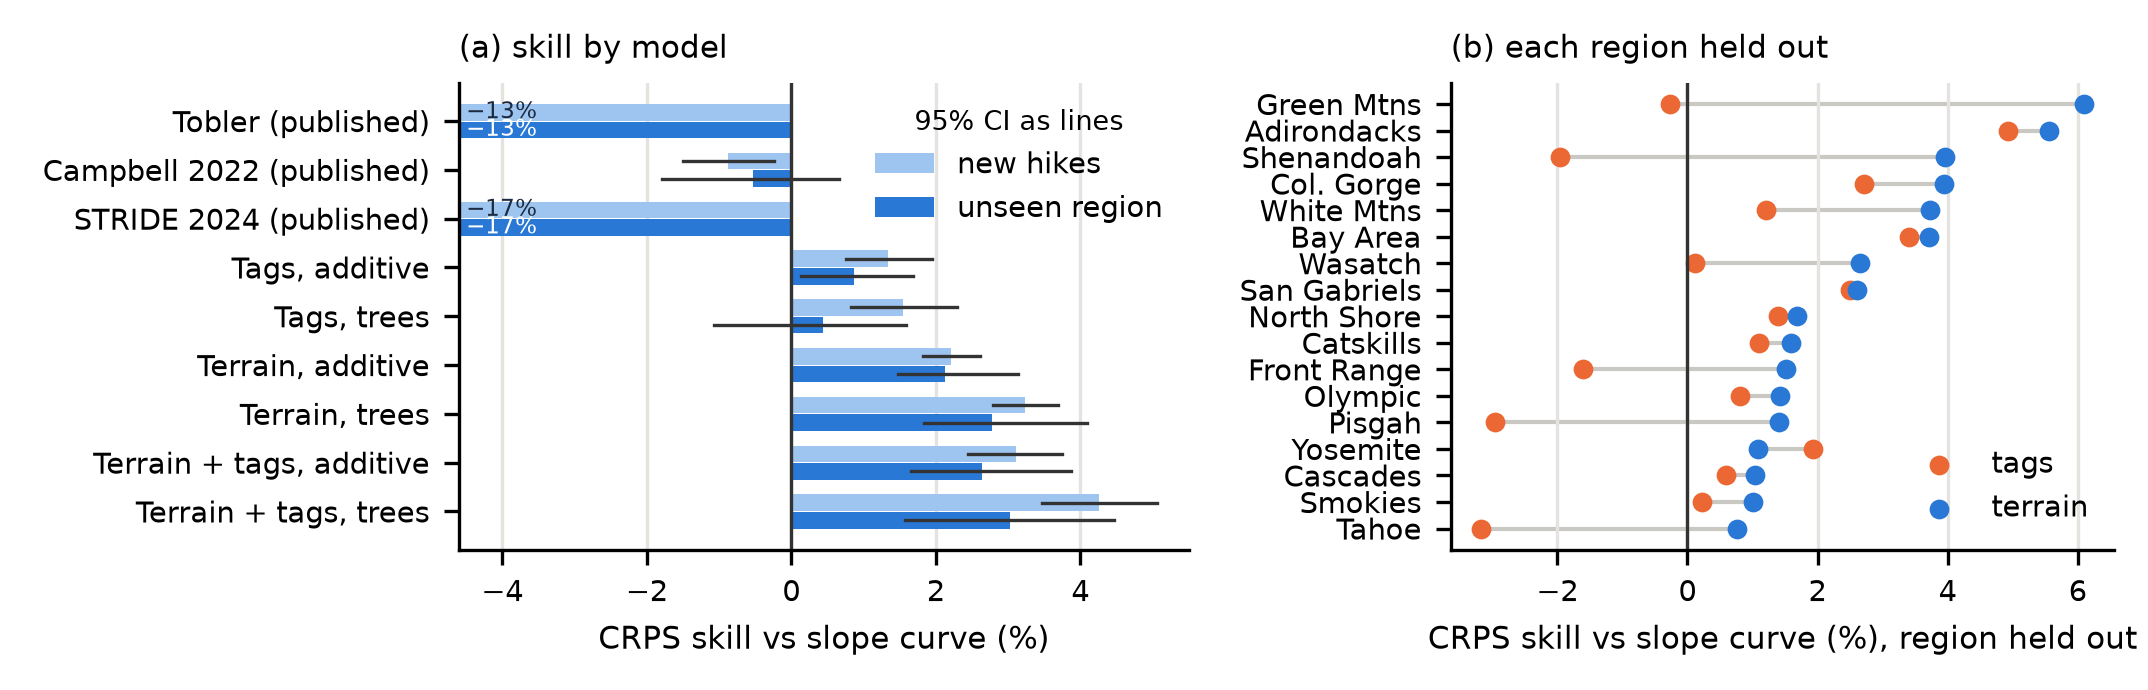
\includegraphics[width=\linewidth]{figures/fig_skill_regions.png}
\caption{CRPS skill over the refitted slope curve (October data, 17 regions). (a)~By model, new hikes (light) and unseen regions (dark). (b)~Each region held out: terrain vs OSM tags.}
\label{fig:skill}
\end{figure}

\begin{table}[t]
\centering
\footnotesize
\setlength{\tabcolsep}{3pt}
\begin{tabular}{@{}lcc@{}}
\toprule
Test & new hikes & unseen regions \\
\midrule
+ imagery A (Clay, landscape) & $+1.03$ [$+0.35$, $+1.71$] & $+0.19$ [$-0.77$, $+1.19$] \\
+ imagery B (Satlas, trail) & $+1.01$ [$+0.57$, $+1.44$] & $+0.16$ [$-0.24$, $+0.57$] \\
\midrule
terrain $-$ tags, 1\,m + 5\,m lidar & & $+1.26$ [$+0.7$, $+2.2$] \\
terrain $-$ tags, 30\,m average & & $+0.83$ [$+0.1$, $+1.4$] \\
terrain $-$ tags, Copernicus & & $-0.68$ [$-1.7$, $+0.2$] \\
\bottomrule
\end{tabular}
\caption{New tests since Report~\#2 (points of CRPS skill, 95\% intervals). Top: gain of terrain + imagery over terrain (trees). Bottom: terrain's lead over tags (additive) by elevation source.}
\label{tab:new}
\end{table}

\paragraph{Imagery (\cref{tab:new}, top).} Track~A used Clay's precomputed NAIP embeddings of 154\,m squares; Track~B embedded 164{,}415 trail-centred 96\,m chips with the frozen Satlas encoder. Both add about one point for new hikes in known regions and nothing reliable in unseen regions, so the pre-set success rule failed. A hand check of 20 chips explains part of it: the trail is visible in only 7, and in none of the 6 eastern forest chips.

\paragraph{Coarse and global elevation (\cref{tab:new}, bottom).} Averaging the 5\,m grids to 10\,m loses nothing, and at 30\,m terrain still beats tags. The real global DEM (Copernicus) does not: along trails it sits 1--19\,m above the lidar ground (canopy), and its slopes are noisier. Terrain needs accurate bare-earth elevation, not fine resolution.

%-----------------------------------------------------------------------------
\section{External Assistance and Collaboration}
\label{sec:help}

My PhD mentors, Danni Beaulieu and Tianyi Gao, meet with me weekly. Danni reviewed the draft with me, pointed out the Bay Area's different sources, and asked for the implementation details now in the paper. Prof.\ Nathan Jacobs is my faculty advisor and will present the paper. Jonathan Lin (MVRL) explained the lab's OSM crawl and its older files. I use Claude (Anthropic), an AI assistant, extensively: it wrote most of the data-processing, modeling and evaluation code, ran the downloads and cluster jobs, drafted the IGARSS paper, and drafted this report from the project's files. I made the scope decisions (dropping the Bay Area, the imagery tracks, the download caps), labelled the chip check, reviewed the results and text, and am responsible for them. Data come from OSM contributors, USGS 3DEP, MRLC, Copernicus (ESA), Google's AlphaEarth, Clay and Microsoft Planetary Computer.

%-----------------------------------------------------------------------------
\section{Reservations and Questions}
\label{sec:questions}

\begin{itemize}\setlength\itemsep{1pt}
\item \textbf{v1.1 numbers.} The data changed by under 2\%, so the conclusions should hold, but every number in the paper must be replaced and checked against the rerun.
\item \textbf{Outside the US.} Terrain's advantage depends on bare-earth elevation; with the free global DEM it disappears. Should the paper say the method needs lidar-quality DEMs, and is there a better global bare-earth product worth one more test?
\item \textbf{Who the hikers are.} OSM uploaders are not a random sample of hikers, and some regions have few traces; I state this as a limit.
\item \textbf{Hardest part now:} rewriting the whole draft in my own words, with the new numbers, in the two weeks before the full draft is due.
\end{itemize}

{\footnotesize
\setlength{\itemsep}{0pt}\setlength{\parskip}{0pt}
\bibliographystyle{ieee_fullname}
\bibliography{refs}
}

\end{document}
